\documentclass[runningheads]{llncs}
\usepackage{graphicx}
\usepackage{hyperref}
\usepackage{stmaryrd}
\usepackage{amsmath}
\usepackage{esvect}
\usepackage{listings}
\usepackage{paralist}
\usepackage{multicol}
\usepackage{subcaption}

% -*- TeX-master: "main.tex" -*-

%%%%%%%%%%%%%%%%%%%%%%%%%%%%%%%%%%%%%%%%%%%%%%%%%%%%%%%%%%%%%%%%%%%%%%%%%%%
% Trace Query Language

\newcommand{\MatchRet}[2]{\textsf{match} \ #1 \ \textsf{return} \  #2}
\newcommand{\FirstAfter}[2]{\textsf{first} \,\ #1 \ \textsf{after} \ #2}
\newcommand{\LastBefore}[2]{\textsf{last} \,\ #1 \ \textsf{before} \ #2}

\newcommand{\Time}[1]{\textsf{time}\SqPar{#1}}
\newcommand{\Rule}[1]{\textsf{rule}\SqPar{#1}}
\newcommand{\IntState}[3]{\textsf{int\_state}\SqPar{#1}\Par{#2, #3}}
\newcommand{\Component}[2]{\textsf{component}\SqPar{#1}\Par{#2}}
\newcommand{\Snapshot}[1]{\textsf{snapshot}\SqPar{#1}}
\newcommand{\AgentId}[1]{\textsf{agent\_id}\Par{#1}}
\newcommand{\Count}[1]{\textsf{count}\Par{#1}}


\newcommand{\TracePat}{P}
\newcommand{\TransPat}{T}

%%%%%%%%%%%%%%%%%%%%%%%%%%%%%%%%%%%%%%%%%%%%%%%%%%%%%%%%%%%%%%%%%%%%%%%%%%%
% Semantics

\newcommand{\Event}[0]{\textsf{Event}}
\newcommand{\Transition}[0]{\textsf{Transition}}
\newcommand{\Matching}[0]{\textsf{Matching}}
\newcommand{\Bool}[0]{\textsf{Bool}}
\newcommand{\Trace}[0]{\textsf{Trace}}
\newcommand{\Value}[0]{\textsf{Value}}
%\newcommand{\Vector}[1]{\vv{#1}}
\newcommand{\Vector}[1]{\vec{#1}}
\newcommand{\At}[2]{{#1}{[#2]}}

\newcommand{\Ag}[0]{\,\textsf{a}}
\newcommand{\Ev}[0]{\,\textsf{E}}
\newcommand{\Tr}[0]{\,\textsf{t}}


\newcommand{\Inter}{\,\cap\,}


\newcommand{\Query}[1]{
\ensuremath{
\arraycolsep=5pt
\def\arraystretch{1.4}
\begin{array}{ll}
#1
}
\end{array}}

%%%%%%%%%%%%%%%%%%%%%%%%%%%%%%%%%%%%%%%%%%%%%%%%%%%%%%%%%%%%%%%%%%%%%%%%%%%
% Maths

\newcommand{\Par}[1]{\left(\, #1  \,\right)}
\newcommand{\SqPar}[1]{\left[\, #1  \,\right]}
\newcommand{\Set}[1]{\left\{\, #1  \,\right\}}
\newcommand{\SetC}[2]{\left\{\, #1 \ | \ #2  \,\right\}}
\newcommand{\Sem}[1]{\left\llbracket \, #1 \, \right\rrbracket}
\newcommand{\Bag}[1]{\Lbag \, #1 \, \Rbag}
\newcommand{\BagC}[2]{\Lbag \, #1 \ | \ #2  \,\Rbag}
\newcommand{\m}[1]{\textsf{#1}}
\newcommand{\OR}[0]{\ \ | \ \ }
\newcommand{\STR}[1]{\texttt{"#1"}}

\newcommand{\MultilineSetC}[3]{
  \ensuremath{
  \def\arraystretch{1.5}
  \begin{array}{ll}
    \{\, #1 \ | \ & #2 \\
    & #3 \,\}
  \end{array}}
}

\newcommand{\LargeMultilineSetC}[3]{
  \ensuremath{
  \def\arraystretch{1.35}
  \Bigg\{
  \, \  #1 \ \ \Big| \ \
  \begin{array}{l}
    #2 \\
    #3
  \end{array}
  \ 
  \Bigg\}
  }
}

\newcommand{\AG}[2]{{#1}\Par{#2}}
\newcommand{\iAG}[3]{#1\!:\!{#2}\Par{#3}}

\newcommand\sbullet[1][.5]{\mathbin{\vcenter{\hbox{\scalebox{#1}{$\bullet$}}}}}
\newcommand{\Free}{\sbullet[.6]}
\newcommand{\Trans}[2]{\, #1 \, \to \, #2 }
\newcommand{\SlashTrans}[2]{\, #1 \, / \, #2 \,}

\newcommand{\StateBefore}[1]{\sbullet[.6]\,{#1}}
\newcommand{\StateAfter}[1]{{#1}\,\sbullet[.6]}



\usepackage{array}

% https://tex.stackexchange.com/questions/12703/how-to-create-fixed-width-table-columns-with-text-raggedright-centered-raggedlef
\newcolumntype{L}[1]{>{\raggedright\let\newline\\\arraybackslash\hspace{0pt}}m{#1}}
\newcolumntype{C}[1]{>{\centering\let\newline\\\arraybackslash\hspace{0pt}}m{#1}}
\newcolumntype{R}[1]{>{\raggedleft\let\newline\\\arraybackslash\hspace{0pt}}m{#1}}


%\newcommand{\BetaCat}{$\textit{Cat}$}
\newcommand{\BetaCat}{\text{Cat}}
\newcommand{\CKOne}{\text{CK1}}
\newcommand{\GSK}{\text{GSK}}




\renewcommand\UrlFont{\color{blue}\rmfamily}

\begin{document}

\title{A Trace Query Language for Rule-based Models}

% \author{Jonathan Laurent\inst{1} \and Jean Yang\inst{1,2}}
\author{Anonymous Authors}

% \authorrunning{Jonathan Laurent et al.}
\authorrunning{Anonymous Authors}


% \institute{Carnegie Mellon University \and Harvard Medical School}\\

\maketitle

%%%%%%%%%%%%%%%%%%%%%%%%%%%%%%%%%%%%%%%%%%%%%%%%%%%%%%%%%%%%%%%%%%%%%%%%%%%

% TODO: novel/unified
\begin{abstract}
  In this paper, we introduce a unified approach for querying
  simulation traces of rule-based models about the statistical
  behavior of individual agents. In our approach, a query consists in
  a trace pattern along with an expression that depends on the
  variables captured by this pattern. On a given trace, it evaluates
  to the multiset of all values of the expression for every possible
  matching of the pattern. We illustrate our proposed query language
  on a simple example, and then discuss its semantics and
  implementation for the Kappa language. Finally, we provide a
  detailed use case where we analyze the dynamics of $\beta$-catenin
  degradation in Wnt signaling from an agent-centric perspective.

  \keywords{Rule-based modeling \and Query Language \and Kappa.}
\end{abstract}

%%%%%%%%%%%%%%%%%%%%%%%%%%%%%%%%%%%%%%%%%%%%%%%%%%%%%%%%%%%%%%%%%%%%%%%%%%%

\section{Introduction}

Rule-based modeling languages such as Kappa \cite{DanosEtAl-CONCUR07}
and BioNetGen \cite{bngl} can be used to write mechanistic models of
complex reaction systems. Models in these languages consist in
stochastic graph-rewriting rules that are equipped with rate constants
indicating their propensity to apply. Together with an initial mixture
graph, these rules constitute a dynamical system that can be simulated
using Gillespie's algorithm
\cite{gillespie1977exact,DanosEtAl-APLAS07,BoutillierEK17}. Each run
of simulation results in a sequence of transitions that we call a
trace.

In practice, simulation traces are often discarded in favor of a
limited number of global features, such
as the concentration curves of a set of observables. However, a more
detailed analysis of their structure and statistical properties can
provide useful insights into a system's dynamics. For example, causal
analysis methods exist
\cite{DanosEtAl-CONCUR07,DBLP:conf/fsttcs/DanosFFHH12} that compress a
large trace into a minimal subset of events that are necessary and
jointly sufficient to replicate an ouctome of interest, and then
highlight causal influences between those remaining events.
% Ideally, such techniques provide a way to uncover signalling
% pathways from networks of low-level protein-protein interactions
Queries about the statistical behavior of individual agents can
lead to complementary insights. Examples include
\begin{inparaenum}[(i)]
\item measuring the average lifespan of a complex under different
  conditions,
\item computing a probability distribution over the states in which a
  particular type of agent can be when targeted by a given rule, and
\item estimating how much of a certain kind of substrate getting
  phosphorylated is due to a particular pathway at different points in
  time.
\end{inparaenum}

In this paper, we propose a unifying language to express queries of
this kind, that are concerned with statistical features of groups of
molecular events that are related in specific motifs. These motifs are
formalized using a notion of \emph{trace pattern}. Then, evaluating a
query comes down to computing the value of an expression for every
matching of a pattern into a trace. We give a first illustration of
this paradigm on a toy example in
section~\ref{sec:starting-example}. After that, we introduce our query
language in section~\ref{sec:semantics} and formalize its semantic
foundations. We then characterize a natural subset of this language
for which an efficient evaluation algorithm exists and discuss our
implementation for the Kappa language
(section~\ref{sec:evaluating-queries}). Finally, we leverage our query
engine to explore aspects of the dynamics of the Wnt signaling
pathway in a detailed use case (section~\ref{sec:use-case}).

% formalize the semantics principle underlying our query language in
% \ref{sec:semantics}.  We

% \ref{sec:evaluating-queries} \ref{sec:use-case}


\section{A Starting Example}\label{sec:starting-example}

In order to illustrate our Trace Query Language, we introduce a toy
Kappa model in Figure~\ref{fig:model}. It is described using a rule
notation that has been introduced in the latest release of the Kappa
simulator and which we borrow in our query language. With this
notation, a rule is described as a pattern that is annotated with
rewriting instructions. The pattern denotes a precondition that is
required for a rule to target a collection of agents. Rewriting
instructions are specified by arrows that indicate the new state of a
site after transformation.

The model of Figure~\ref{fig:model} features two types of agents:
substrates $S$ and kinases $K$. Both kinds of agents have two
different sites, named $x$ and $d$. In addition, $x$-sites can be in
two different internal states: \textit{unphosphorylated} and
\textit{phosphorylated}. We write those states $u$ and $p$,
respectively. Rule $b$ expresses the fact that a substrate and a
kinase with free $d$-sites can bind at rate $\lambda_b$. Rules $u$ and
$u^*$ express the fact that the breaking of the resulting complex
happens at different rates, depending on the phosphorylation state of
the kinase involved. Finally, rule $p$ expresses the fact that a
substrate that is bound to a kinase can get phosphorylated at rate
$\lambda_p$. In all our examples, we consider initial mixtures
featuring free substrates and kinases in smiliar quantity. Substrates
are initially unphosphorylated and kinases are present in both
phosphorylation states.


% -*- TeX-master: "main.tex" -*-
\begin{figure}
  \vspace{-0.2cm}
  \begin{subfigure}[h]{0.4\linewidth}
    \def\arraystretch{1.8}
    \begin{small}
      \begin{tabular}{lllcl}
        \multicolumn{5}{c}{$\lambda_u \gg \lambda_{u^*} \approx \lambda_p$} \\
        $b$ \hspace{0.05cm} & : \hspace{0.1cm} & $ \AG{S}{d^{\Trans{\Free}{1}}}, \ 
        \AG{K}{d^{\Trans{\Free}{1}}} $ &  \ @ \  & $\lambda_b$ \\
        $u$ & : & $ \AG{S}{d^{\Trans{1}{\Free}}}, \ 
                  \AG{K}{d^{\Trans{1}{\Free}}, \ x_u} $ & @ & $\lambda_u$ \\
        $u^*$ & : & $ \AG{S}{d^{\Trans{1}{\Free}}}, \ 
                    \AG{K}{d^{\Trans{1}{\Free}}, \ x_p} $ & @ & $\lambda_{u^*}$ \\
        $p$ & : & $ \AG{S}{d^{\,1}, \  x_{\Trans{u}{p}}}, \ 
                  \AG{K}{d^{\,1}} $ & @ & $\lambda_p$ \\
      \end{tabular}
    \end{small}
    % \subcaption{In Prettified Kappa}
  \end{subfigure}
  \hfill
  \begin{subfigure}[h]{0.46\linewidth}
    \begin{center}
      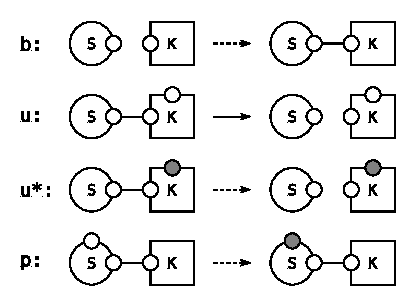
\includegraphics[scale=0.8]{kappa-diagrams/model.pdf}
    \end{center}
    % \subcaption{Graphical Representation}
  \end{subfigure}
  \caption{An Example Kappa Model. On the left, it is described using
    the \textit{edit notation} introduced in KaSim 4. Numbers in a
    rule expression correspond to local bond identifiers and $\Free$
    indicates a free site. Sites not mentioned in a rule are left
    unchanged by it. A graphical representation is provided on the
    right. Phosphorylated sites are indicated in grey. Dotted and
    solid arrows indicate \textit{slow} and \textit{fast} reactions,
    respectively.  }\label{fig:model}
\end{figure}

By playing with this model a bit, one may notice that the
concentration of phosphorylated substrate reaches its maximal value
faster when the ratio of phosphorylated kinases is high (given the
rules of our model, the latter quantity is invariant during
simulation). This phenomenon cannot be explained by looking at rule
$p$ alone. The query provided in~(\ref{eq:exq1}) can be run to
estimate the probability that a substrate is bound to a phosphorylated
kinase when it gets phosphorylated:
\begin{equation}\label{eq:exq1}
  \m{match } t:\Set{ \AG{S}{x_{\Trans{u}{p}},\ d^{\,1}},\ \iAG{k}{K}{d^{\,1}} }
  \, \m{ return } \: \IntState{\StateBefore{t}}{k}{\STR{x}}
\end{equation}
Given a trace, this query matches every transition where a substrate
is getting phosphorylated and outputs the phosphorylation state of the
attached kinase. The variables $t$ and $k$ denote a transition and an
agent, respectively. Moreover, the expression
$\IntState{\,\StateBefore{t}\,}{\,k\,}{\STR{x}\,}$ refers to the
internal state of the site of agent $k$ with name \STR{x} in the
mixture preceding transition $t$.

Running the previous query, we learn that substrates are much more
likely to be phosphorylated by kinases that are phosphorylated
themselves, even when such kinases are in minority in the mixture.
This leads us to conjecture a causal link between the phosphorylation
state of a kinase and its efficiency. After some thoughts, this link
can be easily interpreted: because $\lambda_u \gg \lambda_{u^*}$,
phosphorylated kinases form more stable complexes with substrates,
leaving more chances for a phosphorylation interaction to happen.  In
fact, the average lifespan of a kinase-substrate complex is exactly
$\lambda_{u^*}^{-1}$ when the kinase is phosphorylated and
$\lambda_u^{-1}$ when it is not. We can check these numbers
experimentally by running the following query:
\begin{equation}\label{eq:query-lifespan}
  \Query{
    \m{match} & 
    b:\Set{ \iAG{s}{S}{d^{\Trans{\Free}{1}}}, \ 
      \AG{K}{d^{\Trans{\Free}{1}}, \ x_{p}} } \\
    \m{and} &
    \FirstAfter{u:\Set{ \iAG{s}{S}{d^{\Trans{}{\Free}}} }}{b} \\
    \m{return} & 
    \Time{u} - \Time{b}
  }
\end{equation}
This query outputs a multiset of numbers, whose mean is the average
lifespan of a complex formed by a substrate and a phosphorylated
kinase. The same quantity can be computed for unphosphorylated kinases
by replacing $x_p$ by $x_u$ in the first line
of~(\ref{eq:query-lifespan}).  The pattern in this query does not
match single transitions but pairs of related transitions $(b, u)$,
where $b$ is a binding transition and $u$ the first unbinding
transition to target the same substrate.

\iffalse
% Additional example
\begin{equation}\label{eq:query-kinase-efficiency}
  \Query{
    \m{match} & 
    b:\Set{ \iAG{s}{S}{x_u,\ d^{\Trans{\Free}{1}}}, \ 
      \iAG{k}{K}{d^{\Trans{\Free}{1}}} } \\
    \m{and} &
    \FirstAfter{u:\Set{ \iAG{s}{S}{d^{\Trans{}{\Free}}} }}{b} \\
    \m{return} & 
    \IntState{\StateBefore{b}}{k}{\STR{x}}, \ 
    \IntState{\StateAfter{u}}{s}{\STR{x}}
  }
\end{equation}
\fi

\bigskip

More generally, a query is defined by a {pattern}
$P[\Vec{t}, \Vec{a}]$ and an {expression} $E[\Vec{t}, \Vec{a}]$, which
feature a shared set $\Vec{t}$ of transition variables and a shared
set $\Vec{a}$ of agent variables. The pattern $P$ can be regarded as a
predicate that takes as its arguments a trace $\tau$ and a
\emph{matching} $\phi$ mapping the variables in $\Vec{t}$ and
$\Vec{a}$ to actual transitions and events in $\tau$.  The expression
$E$ can be regarded as a function that maps such $(\tau, \phi)$ pairs
to values. Then, the query evaluates on a trace $\tau$ to the multiset
of all values of $E$, for every matching $\phi$ that satisfies $P$ in
$\tau$.

% TODO: values are tuples, generate a CSV file

\section{The Core Query Language}\label{sec:semantics}

In this section, we introduce the extensible core of our proposed
query language and give it a formal semantics.

\subsection{Meaning and Structure of Queries}\label{subsec:structure}
As shown in Figure~\ref{fig:semantics}, a query $Q$ consists in a
pattern $P$ and an expression $E$. It can be interpreted as a function
$\Sem{Q}$ from traces to multisets\footnote{Note that multisets are
  indicated in Figure~\ref{fig:semantics} using Dijkstra's bag
  notation, whereas sets are indicated using the standard curly
  brackets notation.} of values. The set of allowed values can grow
larger as richer expressions are added to the language. Our current
implementation defines a value as a tuple of base values and features
the following types for base values: \m{bool}, \m{int}, \m{float},
\m{string}, \m{agent}, \m{agent\_set} and \m{snapshot}.

A pattern $P$ is interpreted as a function $\Sem{P}$ that maps a trace
to a set of matchings. A matching $\phi$ is defined by two functions
$\phi_{\Tr}$ and $\phi_{\Ag}$, which map variable names to transition
identifiers and agent identifiers, respectively. We call $\phi_{\Tr}$
a transition matching and $\phi_{\Ag}$ an agent matching.  Given a
trace $\tau$ and a matching $\phi$, the transition variable $v$
denotes the transition $\tau[\phi_{\Tr}(v)]$, where $\tau[i]$ is a
notation for the $i^{th}$ transition of a trace. In addition, an
expression $E$ is interpreted as a function $\Sem{E}$ that maps a pair
of a trace and a matching to a value. The expression language is
extensible and is discussed in section~\ref{subsec:expr-language}. Its
syntax is documented in Figure~\ref{fig:expressions}. Then, the
semantics of a query can be formally defined as follows:
\[ \Sem{\MatchRet{\TracePat}{E}}(\tau) \ = \ \BagC{\Sem{E}(\tau,
    \phi)}{\phi \in \Sem{\TracePat}(\tau) }.  \]

Our language constraints the structure of possible patterns.  As shown
in Figure~\ref{fig:semantics}, a pattern consists in a sequence of
clauses, which can take one of three different forms: $(t:\TransPat)$,
$(\FirstAfter{t:\TransPat}{t'})$ and
$(\LastBefore{t:\TransPat}{t')}$. Here, $t$ and $t'$ are transition
variables and $T$ is a \emph{transition pattern}. In all three cases,
we say that $t$ is \emph{constrained} by the clause.

\subsection{Transition Patterns}\label{subsec:tpats-language}

A transition pattern can be thought as a predicate that takes as its
argument a pair $(\tau, \phi_{\Ag})$ of a transition and an agent
matching. Our current implementation supports specifying transition
patterns using KaSim's \emph{edit notation}. Transition patterns
defined this way are enclosed within curly brackets.  For example, in
query~(\ref{eq:exq1}) of section~\ref{sec:starting-example},
\[ \Set{ \AG{S}{x_{\Trans{u}{p}},\ d^{\,1}},\ \iAG{k}{K}{d^{\,1}} } \]
is true for a transition $t$ and a matching $\phi_{\Ag}$ if and only
if $t$ has the effect of phosphorylating a substrate that is bound to
the kinase with identifier $\phi_{\Ag}(k)$. Formally, a transition
pattern $T$ is interpreted as a function $\Sem{T}$ that maps
transitions into sets of agent matchings. Using the predicate
terminology, one may say that $\phi_{\Ag} \in \Sem{T}(t)$ if and only
if $(t, \phi_{\Ag})$ satisfies $T$.

Our query language can be instantiated with any choice of a language
specifying transition patterns. The only requirement is that
transition patterns should be {decidable efficiently} in the following
sense. Given a transition pattern $T$ and a transition $t$, one should
be able to efficiently compute whether $\Sem{T}(t)$ is empty and
generate an element of it in the case it is not. Our evaluation
algorithm relies on this property.

% TODO: rigidity condition, with clause

\subsection{Expression Language}\label{subsec:expr-language}

We show Figure~\ref{fig:expressions} the syntax of our expression
language. An expression can consist in an agent variable, a constant,
a parenthesized expression, a binary operation, a
function\footnote{Note that functions always take a single argument,
  which can be a tuple.} of an expression, a tuple of expressions or a
\emph{measure}.

Measures are the basic constructs through which information is
extracted from a trace. They come in two different kinds: \emph{state
  measures} and \emph{event measures}. State measures are used to
extract information about the state of the mixture at different points
in the trace. They are parametered with \emph{state expressions} that
can take the form $\StateBefore{t}$ or $\StateAfter{t}\,$, denoting
the states before and after transition $t$, respectively. For example,
the \texttt{int\_state} measure that is used in (\ref{eq:exq1}) is a
state measure. In addition, event measures are used to extract
information that is about a transition itself (in contrast to the
states that it connects). They are parametered by transition
variables. For example, the \texttt{time} measure that is used in
(\ref{eq:query-lifespan}) is an event measure.

The expression language can be easily extended with new operators,
functions, measures and types. In the same way than the language for
specifying transition patterns, it should be regarded as a parameter
of our query language and not as a rigid component.

% TODO: extensible, types, only ask for decidability

% -*- TeX-master: "main.tex" -*-

\begin{figure}[p]
\hrulefill
\centering
\begin{equation*}\label{tql-syntax}
  \arraycolsep=5pt
  \def\arraystretch{1.4}
  \begin{array}{rcclcl}
    \m{query} & Q & := & 
    \MatchRet{\TracePat}{E} \ \, 
    & \ &  \Sem{Q} \in \Trace \to \Bag{\Value} \\
    \m{pattern} & \TracePat & := & C
    & & \Sem{\TracePat} \in \Trace \to \Set{\Matching} \\
    &  & | &  C \,\textsf{and}\, C \\
    \m{clause} & C & := & e:\TransPat
     &  & \Sem{C} \in \Trace \to \Set{\Matching} \\
     &  & | & \FirstAfter{e:\TransPat}{e'} \\
     &  & | & \LastBefore{e:\TransPat}{e'} \\
    \m{event pattern} &  \TransPat & := & \cdots  %\{ M \} \ \textsf{with} \ E
     & & \Sem{\TransPat} \in \Transition \to \Set{\Matching_{\Ag}}  \\
    \m{expression} & E & := & \cdots
     & & \Sem{E} \in \Trace \times \Matching \to \Value \\
  \end{array}
\end{equation*}
\smallskip
\begin{equation*}
    \def\arraystretch{1.9}
    \begin{array}{rcl}
     \Sem{\MatchRet{\TracePat}{E}}(\tau) & \ = \ &
     \BagC{\Sem{E}(\tau, \phi)}{\phi \in \Sem{\TracePat}(\tau)} \\
     % \Sem{C}(\tau) & = & \Sem{C}(\tau) \\
     \Sem{C \m{ and } C'}(\tau) & = & 
     \Sem{C}(\tau) \Inter \Sem{C'}(\tau) \\
     \Sem{ e : P }(\tau) & = & 
     \SetC{\phi}{\phi_{\Ag} \in \Sem{P}(\At{\tau}{\phi_{\Tr}(e)})} \\
  \end{array}
\end{equation*}
\smallskip
\[
 \Sem{ \FirstAfter{e:\TransPat}{e'} }(\tau)  \ = \  
     \LargeMultilineSetC{\phi}{ 
       \phi_{\Ag} \in \Sem{\TransPat}(\At{\tau}{\phi_{\Tr}(e)}) \,,}{
       \forall i. \ \phi_{\Tr}(e') < i < \phi_{\Tr}(e) \implies
       \phi_{\Ag} \notin \Sem{\TransPat}(\At{\tau}{i})
     }
\]
\[
 \Sem{ \LastBefore{e:\TransPat}{e'} }(\tau)  \ = \
     \LargeMultilineSetC{\phi}{ 
       \phi_{\Ag} \in \Sem{\TransPat}(\At{\tau}{\phi_{\Tr}(e)}) \,,}{
       \forall i. \ \phi_{\Tr}(e) < i < \phi_{\Tr}(e') \implies
       \phi_{\Ag} \notin \Sem{\TransPat}(\At{\tau}{i})
     }
\]

\medskip
\hrulefill
\smallskip

\caption{Syntax and semantics of the Trace Query Language}
\label{fig:semantics}
\end{figure} \newcommand{\GEvMeasure}{M_{\textsf{e}}}
\newcommand{\GStMeasure}{M_{\textsf{s}}}


\begin{figure}[p]
  \vspace{0.5cm}
  \hrulefill
  \centering  
  \begin{equation*}\label{expr-syntax}
  \arraycolsep=5pt
  \def\arraystretch{1.4}
  \begin{array}{rccl}
    \m{expression} & E & := &
        a \OR C \OR (\,E\,) \OR E \bowtie E \OR f\,(\,E\,) \OR E\,,\, E \OR \\
     & &  &  
        \GStMeasure[\,S\,] \OR \GStMeasure[\,S\,](\,E\,) \OR
        \GEvMeasure[\,e\,] \OR \GEvMeasure[\,e\,](\,E\,)  \\
    \m{constant} & C & := & 0 \OR 1 \OR \cdots 
          \OR \STR{foo} \,\OR \cdots \\
    \m{binary operator} & \bowtie & := & + \OR - \OR = \OR < \OR \cdots \\
     \m{function} & f & := & 
        \m{agent\_id} \OR \textsf{size} \OR \textsf{count} \OR \cdots \\
    \m{state measure} & \GStMeasure & := & \m{int\_state} \OR
         \m{component} \OR \m{snapshot} \OR \cdots \\
    \m{state expression} & S & := & \StateBefore{e} \OR \StateAfter{e} \\
    \m{event measure} & \GEvMeasure & := & \m{time} \OR
         \m{rule} \OR \cdots \\
    %\m{agent identifier} & a \\
    %\m{event identifier} & e \\
  \end{array}
  \end{equation*}

  {(with $a$ an agent variable and $e$ a transition variable)}

  \medskip
  \hrulefill
  \smallskip

  \caption{Syntax of expressions}
  \label{fig:expressions}
\end{figure}

\section{Evaluating Queries}\label{sec:evaluating-queries}

In this section, we introduce a natural subset of the language
described in section~\ref{sec:semantics}, for which we provide an
efficient implementation. Queries in this subset are said to be
\emph{regular}, and they display an interesting {rigidity} property.

\subsection{Rigidity}

Intuitively, a pattern is said to be rigid if its matchings are
completely determined by the value of a single transition variable.
\begin{definition}\label{def:rigidity}
  Given a Kappa model, a pattern $P$ is said to be \emph{rigid} if and
  only if it features a transition variable $r$ called \emph{root
    variable} such that for any trace $\tau$ that is valid in the
  model, we have
  \[ \forall\, \phi, \phi' \in \Sem{P}(\tau), \ \phi_{\Tr}\,(r) =
    \phi'_{\Tr}\,(r) \implies \phi = \phi'. \]
\end{definition}
For example, the pattern $P$ of query~(\ref{eq:query-lifespan})
% in section~\ref{sec:starting-example}
is rigid, with root variable $b$. Indeed, suppose that $b$ is matched
to a specific transition $t$. Then, the agent variable $s$ is
determined by $t$ as no more than one substrate can get bound during a
single transition given the rules of our model
(Figure~\ref{fig:model}). Finally, $u$ is uniquely determined as the
first unbinding event that targets $s$ after $b$.

An easy consequence of Definition~\ref{def:rigidity} is that the
number of matchings of a rigid pattern into a trace is bounded by the
size of this trace.

\subsection{Regular Queries}

Our evaluation algorithm handles a subset of queries whose patterns
admit a certain tree structure. For those patterns, rigidity is
implied by a weaker notion of \emph{local rigidity}.
\begin{definition}
  Given a Kappa model, a transition pattern $T$ is said to be
  \emph{rigid} if and only if for any agent variable $a$ that appears
  in $T$ and every valid transition $t$, we have
  \[ \forall\, \phi_{\Ag}\,, \phi_{\Ag}' \in \Sem{T}, \ \phi_{\Ag}(a)
    = \phi'_{\Ag}(a). \]
\end{definition}
Intuitively, a transition pattern is rigid if matching it to a
transition determines all its agent variables.
\begin{definition}
  Given a model, a pattern $P$ is said to be \emph{locally rigid} if
  it features only rigid transition patterns. Then, a transition
  variable $t$ is said to \emph{determine} an agent variable $a$ if
  there is a clause of $P$ that constrains\footnote{As defined in
    section~\ref{subsec:structure}.} $t$ and features $a$.
\end{definition}
For patterns with a particular structure, local rigidity implies
rigidity. This structural assumption can be expressed in terms of a
pattern's \emph{dependency graph}.
\begin{definition}
  The \emph{dependency graph} of a pattern $P$ is a graph whose nodes
  are the transition variables of $P$ and for which there is an edge
  from $t$ to $t'$ if and only if $P$ contains a clause of the form
  % \[\FirstAfter{t':T}{t} \qquad \text{or} \qquad
  %   \LastBefore{t':T}{t}.\]
  $(\FirstAfter{t':T}{t})$ or $(\LastBefore{t':T}{t})$.
\end{definition}
We can now define the notion of a regular pattern, and thus of a
regular query.
\begin{definition}\label{def:regularity}
  A pattern is said to be \emph{regular} if the following three
  conditions hold:
  \begin{inparaenum}[(i)]
  \item\label{reg:locally-rigid} it is locally rigid
  \item\label{reg:tree} its dependency graph is a tree
  \item\label{reg:well-captured} whenever two of its transition
    variables determine a same agent variable, one of them has to be a
    descendent of the other in the dependency tree.
  \end{inparaenum}
\end{definition}
This structure enables an efficient enumeration of the matchings of a
regular pattern into a trace. Moreover, the number of these matchings
is bounded by the size of the trace, as regular patterns can be proven
to be rigid.
\begin{proposition}\label{prop:regular-rigid}
  Regular patterns are rigid.
\end{proposition}
Finally, regular queries are defined as expected.
\begin{definition}
  A query is said to be \emph{regular} if its pattern is regular.
\end{definition}
This notion of regularity may appear unintuitive at first, and we
agree that its formal definition is somewhat involved. However, we
argue that regular queries are exactly those queries that admit a
natural operational interpretation. Therefore, experimentalists tend
to think in terms of regular queries instinctively.

% More precisely, the root of the dependency tree of a regular pattern
% is a root variable, in the sense of
% Definition~\ref{def:rigidity}. The intuition underlying this
% proposition should become clearer in section~\ref{subsec:evalq},
% when we introduce an algorithm for evaluating regular queries
% (defined below).

\subsection{Evaluating Regular Queries
  Efficiently}\label{subsec:evalq}

When designing an algorithm for evaluating trace queries, one has to
keep in mind that the corresponding sequence of state mixtures cannot
fit in random-access memory all at once, even for small traces. In
fact, even the most economic representation of a trace, which is
specified by an initial mixture and a sequence of labeled rewriting
events, may fail to fit in memory in some cases. Therefore, as often
as possible, one should only be allowed to stream such a
representation from disk, recomputing intermediate states dynamically
and never keeping more than a small number of them in memory at once
(two in our case).

Our algorithm for evaluating a regular query proceeds in two
steps. First, it streams the trace to compute the set of all matchings
of the pattern. Then, it streams the trace a second time to compute
the value of the expression for all these matchings. The second step
is quite simple to implement. Indeed, once the matchings are known, it
is easy to compute the sequence of all measures that need to be
performed and order them in increasing order of time. The first step
attempts to match the root variable of the pattern to every transition
in the trace. For each candidate matching, it uses rigidity to
determine all other variables progressively as the trace is streamed,
in an order that is determined by the dependency tree and with a
minimal amount of caching. Overall, the algorithm runs in time linear
in the length of the trace.


\subsection{Our Implementation}

We provide an implementation of our proposed trace query language,
which relies on the algorithm that is mentioned in
section~\ref{subsec:evalq} for evaluating regular queries. Our query
engine takes for inputs
\begin{inparaenum}[(i)]
\item a file that contains a list of queries written in the same
  syntax that we use in our examples and
\item a trace file that has been generated by the Kappa simulator
  using the \texttt{-trace} option.
\end{inparaenum}
It evaluates all queries at once and generates one output file per
query, in comma-separated values (CSV) format.\footnote{Every line of
  an output file represents a single value. In our expression
  language, values are tuples of \emph{base values}. These are
  separated by commas within a line.}

Queries that are non-regular for structural reasons -- i.e. that fail
to meet criterion (\ref{reg:tree}) or (\ref{reg:well-captured}) of
Definition~\ref{def:regularity} -- are rejected immediately.  As there
is no easy static check for local rigidity,
% -- criterion (\ref{reg:locally-rigid}) --
queries that do not meet this criterion will be rejected at runtime.
% In both cases, informative error messages are generated.

\medskip

We now introduce a use case in which we leverage our query engine to
explore aspects of the dynamics of the Wnt signaling pathway.


\iffalse
However, the first users of our query engine never expressed any
frustration with it, as they naturally came up with regular queries
only.\footnote{Furthermore, they would also write the clauses of their
  patterns in an order that reflects their dependency trees.}  In our
opinion, this is due to the difficulty of interpreting non-regular
queries operationally.
\fi


%We provide an implementation

% How non regular are rejected ?
% CSV

\newpage 

\section{A Use Case on Wnt Signaling}\label{sec:use-case}

In this use case, we are focusing on a simplified model of the
$\beta$-catenin destruction complex from canonical Wnt signaling. This
complex is highly conserved in animals, and operates from humans to
nematodes to insects to amphibians, regulating the establishment of
the dorso-ventral axis. It is also heavily involved in colon cancer.

A source of complexity in our model is the fact that none of the
enzymes involved in destroying $\beta$-catenin bind it directly.
Instead they are loaded onto a scaffold. Moreover, the scaffold can
head-to-tail homopolymerize, in addition to having three independent
binding sites on a second scaffold, itself capable of dimerization.
This allows a complex of scaffolds, where connection
paths or stoichiometries are dynamic. It is this complex that acts as a
super-scaffold to bring the substrate in contact with the
enzymes. Considering both scaffolds contain large regions of disorder
(i.e. chunks of unfolded peptide with high flexibility), it is
sensible to believe an enzyme loaded on one scaffold could modify the
substrate loaded on the neighboring scaffold. Lacking experimental
evidence to suggest a ballpark limit for this reachable horizon, we
leave it unconstrained: an enzyme will be able to modify any substrate
loaded onto its complex.

Another source of complexity is that having kinases (i.e. enzymes that
add a phosphate group) and phosphatases (i.e. enzymes that remove a
phosphate group) loaded on the same complex will result in
unimolecular do-undo loops. Conceivably the kinetics of complexes will
vary heavily with the amount of kinases, phosphatases, and substrates
loaded onto them. %These are all dynamic properties.

\bigskip

We leverage our trace query engine to explore the dynamics of this
system. More precisely, we develop queries to probe the agent-centric
dephosphorylation dynamics, to measure the time it takes for an agent
to navigate the modification steps, and to explore the complexes at
which events happen.

Our results are relevant to other pathways in addition to Wnt, from
NF$\kappa$B to RAS/ERK to the most studied protein on the world, P53;
the pathways these proteins regulate make heavy use of polymeric
scaffold complexes, sequential modifications, and do-undo loops.




\subsection{Experimental Protocol and Queries}

To explore our system, we create a Kappa model with three
parametrizations. The model contains the scaffold proteins Axin1 (Axn)
and APC, the kinases CK1$\alpha$ (CK1) and GSK3$\beta$ (GSK), the
protein phosphatases PP1 and PP2, and the substrate of all these
reactions, $\beta$-catenin (Cat). The destruction complex recruits
Cat through Axn. It then gets phosphorylated at the Serine on position
45 (S45) by CK1. While S45-phosphorylated, it can be phosphorylated at
the Threonine on position 41 (T41) by GSK. While T41-phosphorylated,
it can be phosphorylated on both Serines on positions 37 and 33 (S37 and
S33). Once S37- and S33-phosphorylated, Cat is degraded. Meanwhile, PP1
undoes the phosphorylations of CK1, while PP2 undoes those of GSK. Each
kinase-phosphatase pair also compete against each other for binding sites
on Axn.

The three parametrizations explore the relationship
between phosphatase/kinase ratio and the distribution of do-undo
events. The three parameter pairs are 50/10, 10/10, and
10/50, all in units of number of agents, and represent the number of kinases and
phosphatases in the model (e.g. 10/50 presents 10 copies of PP1, 10
copies of PP2, 50 copies of CK1, and 50 copies of GSK). The scaffolds
remain at an abundance of 100 each. The models begin with an initial
amount of Cat of 500 agents, and the models are run for 500
simulated seconds. We use global stochastic rates for our reactions, a bi-molecular binding of $10^{-4}$ per second per agent, a uni-molecular binding of $10^{-2}$ per second, an unbinding of $10^{-2}$ per second, and a catalytic of $1.0$ per second.

For all three parametrizations, we run the following queries on the
resulting traces.

%%%%%%%%%%%%%%%%%%%%%%%%%%%%%%%%%%%%%%%%%%%%%%%%%%%%%%%%%%%%%%%%%%%%%%%%%%%%%%%%

\subsubsection*{Undoing S45, T41, S37 and S33 phosphorylation}
Considering phosphatases undoing the phosphorylation of
sites, does this happen to all agents? Does it happen to just a few agents? What is the distribution of dephosphorylation events per agent? (Figure~\ref{F1})

%match e:{c:Cat(S45{ph/un})}
%return (agent_id{c}, time[e])

%match e:{c:Cat(T41{ph/un})}
%return (agent_id{c}, time[e])

%match e:{c:Cat(S37{ph/un})}
%return (agent_id{c}, time[e])

%match e:{c:Cat(S33{ph/un})}
%return (agent_id{c}, time[e])

\newcommand{\UndoQ}[1]{
\Query{
    \m{match} & e:\Set{ 
      \iAG{c}{\BetaCat}{{#1}^{\,1}_{\Trans{p}{u}}}
    } \\
    \m{return} & \AgentId{c},\, \Time{e}
  }
}

\begin{small}
  \begin{equation*}
    \arraycolsep=7pt
    \begin{array}{cc}
      \UndoQ{S45} & \UndoQ{T41} \\ \\
      \UndoQ{S37} & \UndoQ{S33} \\
    \end{array}
  \end{equation*}
\end{small}

%%%%%%%%%%%%%%%%%%%%%%%%%%%%%%%%%%%%%%%%%%%%%%%%%%%%%%%%%%%%%%%%%%%%%%%%%%%%%%%%

\subsubsection*{Wait times}

What is the distribution of times spent
between the first phosphorylation on an agent, and the time it gets
degraded? (Figure~\ref{F2})

%match i:{+c:Cat}
%and first p:{c:Cat(S45{un/ph})} after i
%and first d:{-c:Cat} after p
%return (agent_id{c}, time[p], time[d])

\begin{small}
\begin{equation}
  \Query{
    \m{match} & i:\Set{  c:\BetaCat+ } \\
    \m{and} & \FirstAfter{p:\Set{
        \iAG{c}{\BetaCat}{{S45}_{\Trans{u}{p}}}
    }}{i} \\
    \m{and} & \FirstAfter{ d:\Set{
        c:\BetaCat-
    } }{p} \\
    \m{return} & \Time{d} - \Time{p}
  } 
\end{equation}
\end{small}

\noindent \textit{About this query.} Agent creation and destruction is
expressed by suffixing agent names with $+$ and $-$,
respectively.

%%%%%%%%%%%%%%%%%%%%%%%%%%%%%%%%%%%%%%%%%%%%%%%%%%%%%%%%%%%%%%%%%%%%%%%%%%%%%%%%

\subsubsection*{Component size and enzyme identity} 
Where do the phosphorylation steps that actually lead to degradation
occur? Do they happen mostly on large complexes? What is
the composition in units of Axn and APC of the complexes where the
phosphorylation events leading to degradation took place? What is the distribution of kinase identifiers for the last phosphorylation events that lead to degradation? (Figure~\ref{F6})

\newcommand{\BigHectorStoryLine}[4]{
\LastBefore{#1:\Set{ 
          \iAG{c}{\BetaCat}{ {#2}^{\,1}_{\Trans{u}{p}}}, \ 
          \iAG{#3}{#4}{c^{\,1}}
    }}{d}
}
\newcommand{\BigHectorStoryRet}[2]{
\AgentId{#2}, \ \Count{ \Component{\StateBefore{#1}}{#2}, \, 
      \STR{Axn}, \, \STR{APC} }
}

%match d:{-c:Cat}
%and last p1:{ c:Cat(S45{un/ph}[1]), k1:CK1(c[1])} before d
%and last p2:{ c:Cat(T41{un/ph}[1]), k2:GSK(c[1])} before d
%and last p3:{ c:Cat(S37{un/ph}[1]), k3:GSK(c[1])} before d
%and last p4:{ c:Cat(S33{un/ph}[1]), k4:GSK(c[1])} before d
%return (
%	agent_id{k1}, count{'Axn', 'APC'}{component[.p1]{k1}},
%	agent_id{k2}, count{'Axn', 'APC'}{component[.p2]{k2}},
%	agent_id{k3}, count{'Axn', 'APC'}{component[.p3]{k3}},
%	agent_id{k4}, count{'Axn', 'APC'}{component[.p4]{k4}}

\begin{small}
\begin{equation}
  \Query{
    \m{match} & d:\Set{ c:\BetaCat - } \\
    \m{and} & \BigHectorStoryLine{p_1}{S45}{k_1}{\CKOne} \\
    \m{and} & \BigHectorStoryLine{p_2}{T41}{k_2}{\GSK}   \\
    \m{and} & \BigHectorStoryLine{p_3}{S37}{k_3}{\GSK}   \\
    \m{and} & \BigHectorStoryLine{p_4}{S33}{k_4}{\GSK}   \\
    \m{return} 
    & \BigHectorStoryRet{p_1}{k_1} \,,\  \\
    & \BigHectorStoryRet{p_2}{k_2} \,,\ \\
    & \BigHectorStoryRet{p_3}{k_3} \,,\  \\
    & \BigHectorStoryRet{p_4}{k_4} \\
  }
\end{equation}
\end{small}

\noindent \textit{About this query.} The \textsf{component} state
measure computes the connected component that contains an agent in a
mixture. It returns a set of agents $S$. The \textsf{count} function
takes such a set $S$ along with $n$ strings denoting agent types and
returns an $n$-tuple of integers indicating how many agents of each
type appear in $S$.



\subsection{Results and Interpretation}

\subsubsection*{Distribution of undo events per agent}

To study the effect of adding phosphatase, we look at the distribution
of dephosphorylation events per agent in Figure~\ref{F1}. S45 is the
first residue to be modified in the causal chain leading to
degradation; S37 is the last. Based on the 1:1 system, it is surprising
to see increasing the phosphatase level five-fold maintains a similar
total number of dephosphorylation events (compare curves' integrals).
However, their distribution is quite different. Interestingly,
increasing the amount of kinase to 1:5 led to decrease in
dephosphorylation events, even though the dephosphorylation enzyme's
abundance and rates were kept at the same levels. It is also worth
noting, the 1:1 saw almost 30 thousand dephosphorylation events of
S45, occurring on a shrinking pool of at most 500 copies of Cat.
Clearly certain agents are caught in the do-undo loop; some specific
agents are getting dephosphorylated almost 800 times. It is worth
noting these levels of dephosphorylation imply a comparable number of
phosphorylation events.

To answer the question that motivated this query, for S45 under 1:5 regime,
most agents don't get sabotaged by the phosphatase: the blue line is
quite flat. Decreasing the amount of kinase changes this, and
under a 1:1 regime some agents get undone multiple times, a quarter
seeing upwards of hundreds of undo events (e.g. from id 300
onward). Increasing the phosphatase to a 5:1 regime further
exacerbates this, with over half the agents receiving undo events
hundreds of times. The unavailability of phosphorylated S45 in turn
inhibits the phosphorylation of T41, and so forth to S37 and S33. It
is worth noting that, based on the 1:1 system, \emph{increasing} the
phosphatase five-fold \emph{decreases} the number and extent of advanced
dephosphorylation events, such as S33 and S37. Paradoxically,
increasing the kinase five-fold has this same effect. We attribute the
former to decreased availability of the intermediate phosphorylated
states (i.e. if T41 is not phosphorylated, S37 can't be
phosphorylated, ergo can't be dephosphorylated), and the latter to
increased throughput to degradation (i.e. Cat is not around for long
enough to get dephosphorylated, as once it gets fully phosphorylated it
quickly proceeds to get degraded).

We call attention to the number of agents whose final sites got
dephosphorylated (Figure~\ref{F1}), vs. the number of agents who got
degraded (Figure~\ref{F0}, in Appendix~\ref{ap:use-case}). The 1:5 or
1:1 systems both degraded over 450 agents each, but the former undid
around 160 agents (Figure~\ref{F1} S37, domain of blue curve) while
the latter undid over 350 (Figure~\ref{F1} S37, domain of red
curve). For the 1:5 and 5:1 systems, both undid around 160 agents
(Figure~\ref{F1} S37, domain of blue and yellow curves), but the
former degraded over 450 agents (Figure~\ref{F0}, blue curve) while
the latter less than 50 (Figure~\ref{F0}, yellow curve). This argues
the notion of efficiency (e.g. minimizing the amount of undo steps)
can't readily be inferred from the throughput of the system.


\begin{figure}[h]
  \centering
  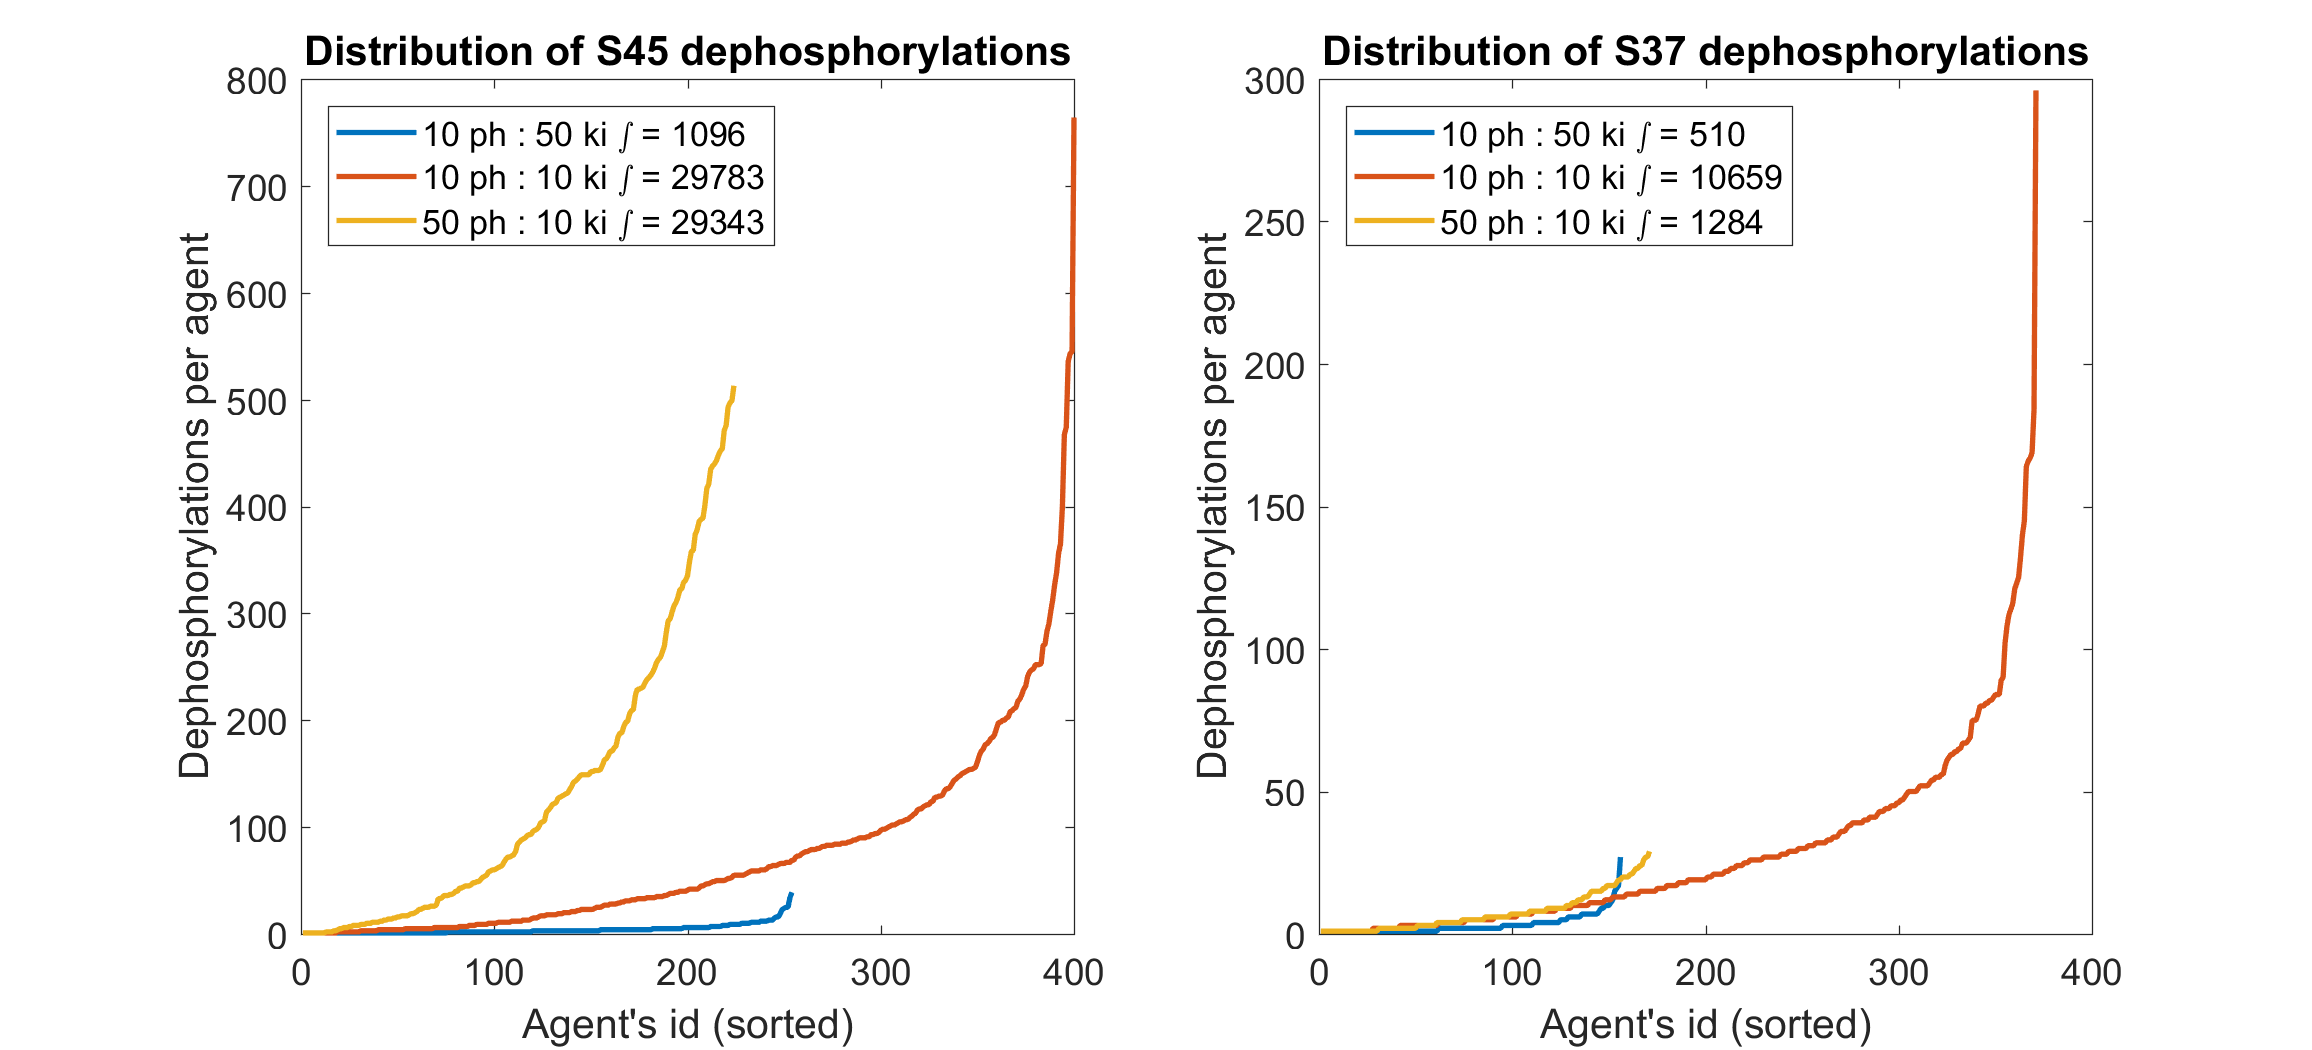
\includegraphics[width=\columnwidth]{wnt/F1_distribution_dephosphorylations_per_agent_brief.png}
  \caption{Distribution of dephosphorylation events per agent. Each
    time an agent gets dephosphorylated, its ID is registered. After
    sorting, we plot the distribution of these IDs for two residues in
    the three parameter regimes. The area under the curve is also
    presented on each legend. S45 is the first residue to get
    phosphorylated, S37 (along with S33) is the last.}
  \label{F1}
\end{figure}


\subsubsection*{Wait times}
Looking at the distribution of wait times (Figure~\ref{F2}), from
first phosphorylation to degradation, we note the bulk of degradation
events occur rapidly, in less than $50$ seconds. Worth noting that,
from the 1:1 regime, increasing the amount of kinase five-fold
marginally reduced wait times.

\begin{figure}[h]
  \centering
  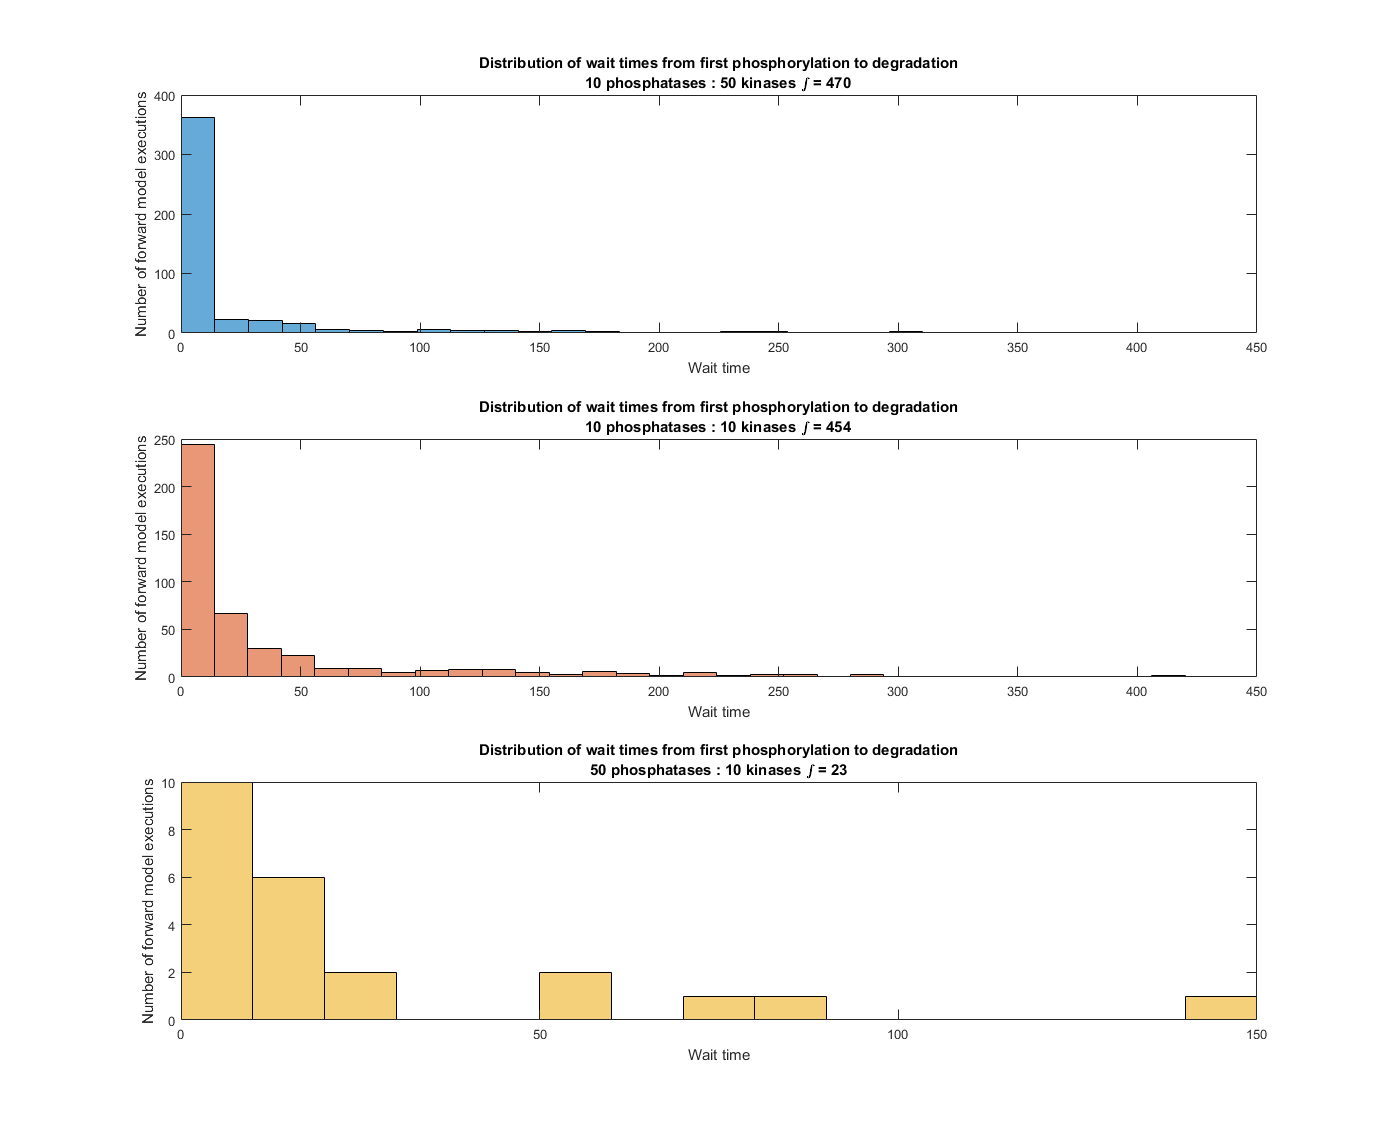
\includegraphics[width=\columnwidth]{wnt/F2_wait_times.png}
  \caption{Distribution of wait times from first phosphorylation until
    degradation. The sum of the bins is presented in the legend of
    each plot, and corresponds to the total number of degradation
    events, matching what is seen on Figure~\ref{F0}. The height of
    each bin represents the number of agents that waited the bin's
    position (in seconds) since they were first modified until they
    were degraded.}
  \label{F2}
\end{figure}


\subsubsection*{Complex composition}

A way of looking at the question of complex contribution is to query
the size of the complex at the last phosphorylation event before
degradation. Taking S45 as representative of all the other residues
(see Figure~\ref{F11} in Appendix~\ref{ap:use-case} for a residue comparative),
we plot the size of the complex, in terms of Axn and APC, at the time
the final S45 occurred. Overall, we see a broad distribution of sizes,
with some phosphorylation events occurring in large complexes
(i.e. $>80$ Axn, $>40$ APC), but a significant number occurring in far
smaller complexes (i.e. $<10$ Axn, $<10$ APC). Changing the parameter
regime of kinase to phosphatase does not seem to alter this behavior
significantly.

\begin{figure}[h]
  \centering
  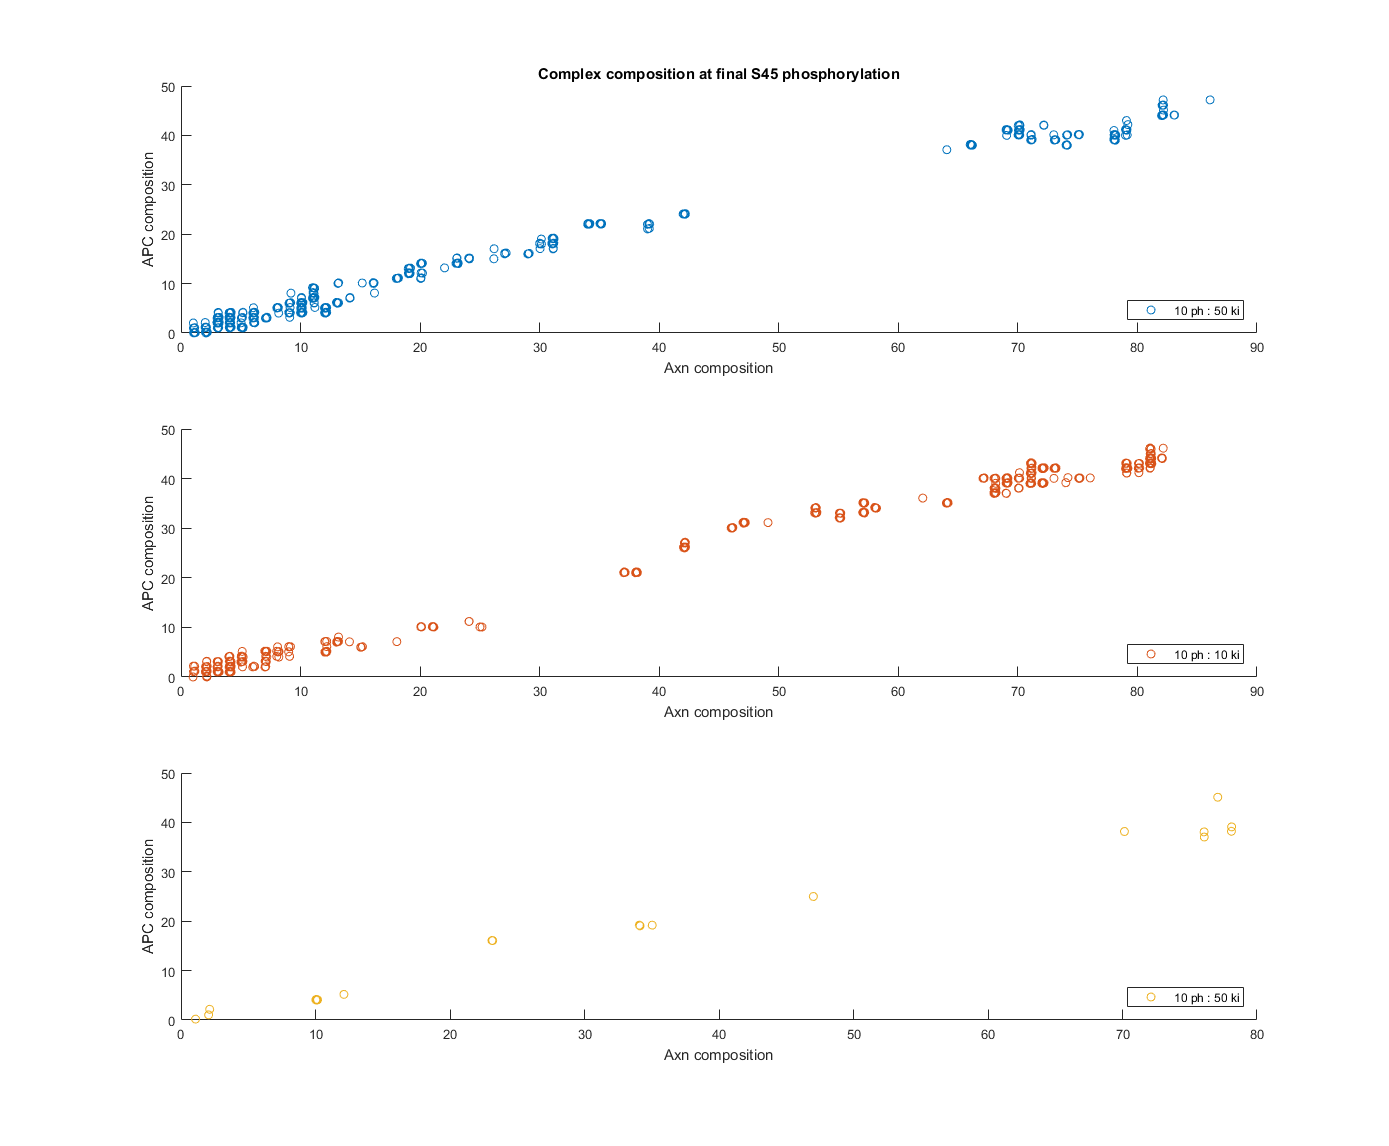
\includegraphics[width=\columnwidth]{wnt/F6_complex_composition_final_S45.png}
  \caption{Composition of the complex, in terms of Axn and APC
    components, at the last event where Cat got S45 phosphorylated
    before being degraded. The number of points corresponds to the number of
    degradation events. The points of this scatter plot have
    been nudged with a random noise factor of 0.2 to increase visual
    perception of discrete points where the data overlap.}
  \label{F6}
\end{figure}


\subsection{Summary of Findings}

\begin{enumerate}
\item The number of undo events does not inform us of overall
  throughput (contrast Figure~\ref{F1} and Figure~\ref{F0}).
\item How a step may be affected by changing abundances depends
  greatly on its upstream context (Figure~\ref{F1}).
\item Entities that got degraded waited a short while since their
  first modification (Figure~\ref{F2}), and yet most modifications
  were futile (Figure~\ref{F1}).
\item We can't argue that giant complexes, nor small complexes, nor
  medium complexes, are the sole entities responsible for performing
  the effective (i.e. final) phosphorylation events  (Figure~\ref{F6}); %F6-9
  the distribution of complexes is wide, and they all contribute to
  the kinetics.
\end{enumerate}

The capacity of querying a simulation's trace offers a mechanistic description of the inner workings of our system. Since this description uses the vocabulary of molecular biology, it can greatly inform the search for drug targets. 

For example, in our setup, complexes with over 60 copies of Axn and over 40 copies of APC contributed a large amount of degradation events (Figure~\ref{F6}). Considering there were a total of 100 copies of each scaffold, these large complexes are giant components, having recruited the majority of scaffolds into a single entity. If a single entity is contributing an amount of degradation events comparable to the rest of the mixture, it means its \emph{effective} catalytic rate is greater than that of smaller entities. One could therefore reduce overall degradation of Cat by destabilizing any of the three scaffold interactions (i.e. Axn-Axn, APC-APC, Axn-APC), without affecting the enzymes directly. Since these enzymes are also involved in metabolism, it would be desirable to avoid affecting their behaviors outside our pathway of interest.

\bigskip

Beyond Wnt, our approach can serve to add an analytical dimension to the phase-transition model suggested by Pronobis et al \cite{pronobis2017reconstituting}. If the mixture transitions from an fragmented regime into an aggregated one, the aggregated regime is expected to enjoy greater local concentrations of enzymes and substrates within the large components. Through our trace query language, we can assay the size of components as they contribute catalytic events. This allows us to quantify the degradation activity inside and outside the distinct phases by querying the size of the scaffold complex at the times of enzymatic modifications. Were one to make a model of the specific setup and chimeric protein of Pronobis et al, we would expect the distribution of events to reveal the distinct phases suggested by the authors.

Our trace query language could also aid in the characterization of the \emph{aggregate-with-tentacles} model of Anvarian et al \cite{anvarian2016axin}. The gain-of-function mutations identified by the authors create novel binding capacities. By distinguishing bi-molecular from uni-molecular interactions, one can model local concentration effects. Specifically, one can model the effect of having novel binding sites on the complex' \emph{tentacles}, in close proximity by nature of being loaded on the same complex. One can therefore model the growth of the complex as additional binding sites become active (e.g. by setting a binding rate to greater than zero). Were one to make a model informed by the specific experimental setup used by the authors, one could quantify the change in unbound state as additional binding sites become active.

% Say a few words about the speed of the implementation

\newpage

\section{Conclusion}

How could one have explored a question like ``which complexes
contribute to kinetics''? Experimental biologists have been using
labeling techniques for decades, but implementing this in a modeling
framework requires being able to track individual agents, and query
particular events. Implementing a framework to query events on the
trace of an agent and rule simulation seems a natural way of tackling
these classes of problems. Moreover, once a sufficiently rich
\emph{mechanistic} model is available, questions on \emph{mechanism}
arise. For a subset of these, a satisfying answer will require a
change of vocabulary; the explanations desired use the individual's
lexicon (e.g. it bound, it unbound, it got dephosphorylated 800
times), rather than a whole system lexicon (e.g. the abundance changed
from 500 to 50). Thus, rather than tracking the whole model's behavior
(akin to a top-down approach), one needs to focus on agents, and
observe their individual experiences (akin to a bottom-up
approach). These approaches are complementary, as they explore a
model's intricacies from very different viewpoints. We hope that the
query language proposed in this paper will contribute to make
agent-centric analyses more widespread and accessible.



% Interaction with causal analysis Insist on the clean semantics
% foundations Natural queries are natural

% \input{playground.tex}

% Extensions and Future work

%%%%%%%%%%%%%%%%%%%%%%%%%%%%%%%%%%%%%%%%%%%%%%%%%%%%%%%%%%%%%%%%%%%%%%%%%%%
% ---- Bibliography ----

\nocite{*} \bibliographystyle{splncs04} \bibliography{main}

\newpage

\appendix

\subsection*{Use Case Appendix}

\subsubsection*{Concentration Time Traces}
From the simulator�s output, we get the evolution of the abundance of
Cat through time. In Figure~\ref{F0}, we can see the systems with low phosphatase
behave similarly, even though one has five times the amount of kinases
than the other (blue vs red traces). In contrast, the system with high
phosphatase shows markedly less degradation of Cat; where the other
two system degraded around 450 units, this one has only degraded
23. From this whole-system view, it would seem the amount of
phosphatase is more critical than the amount of kinase: based on the
1:1 system, increasing the kinase five fold has little effect, whereas
increasing the phosphatase has a more dramatic effect.

\begin{figure}[p]
  \centering
  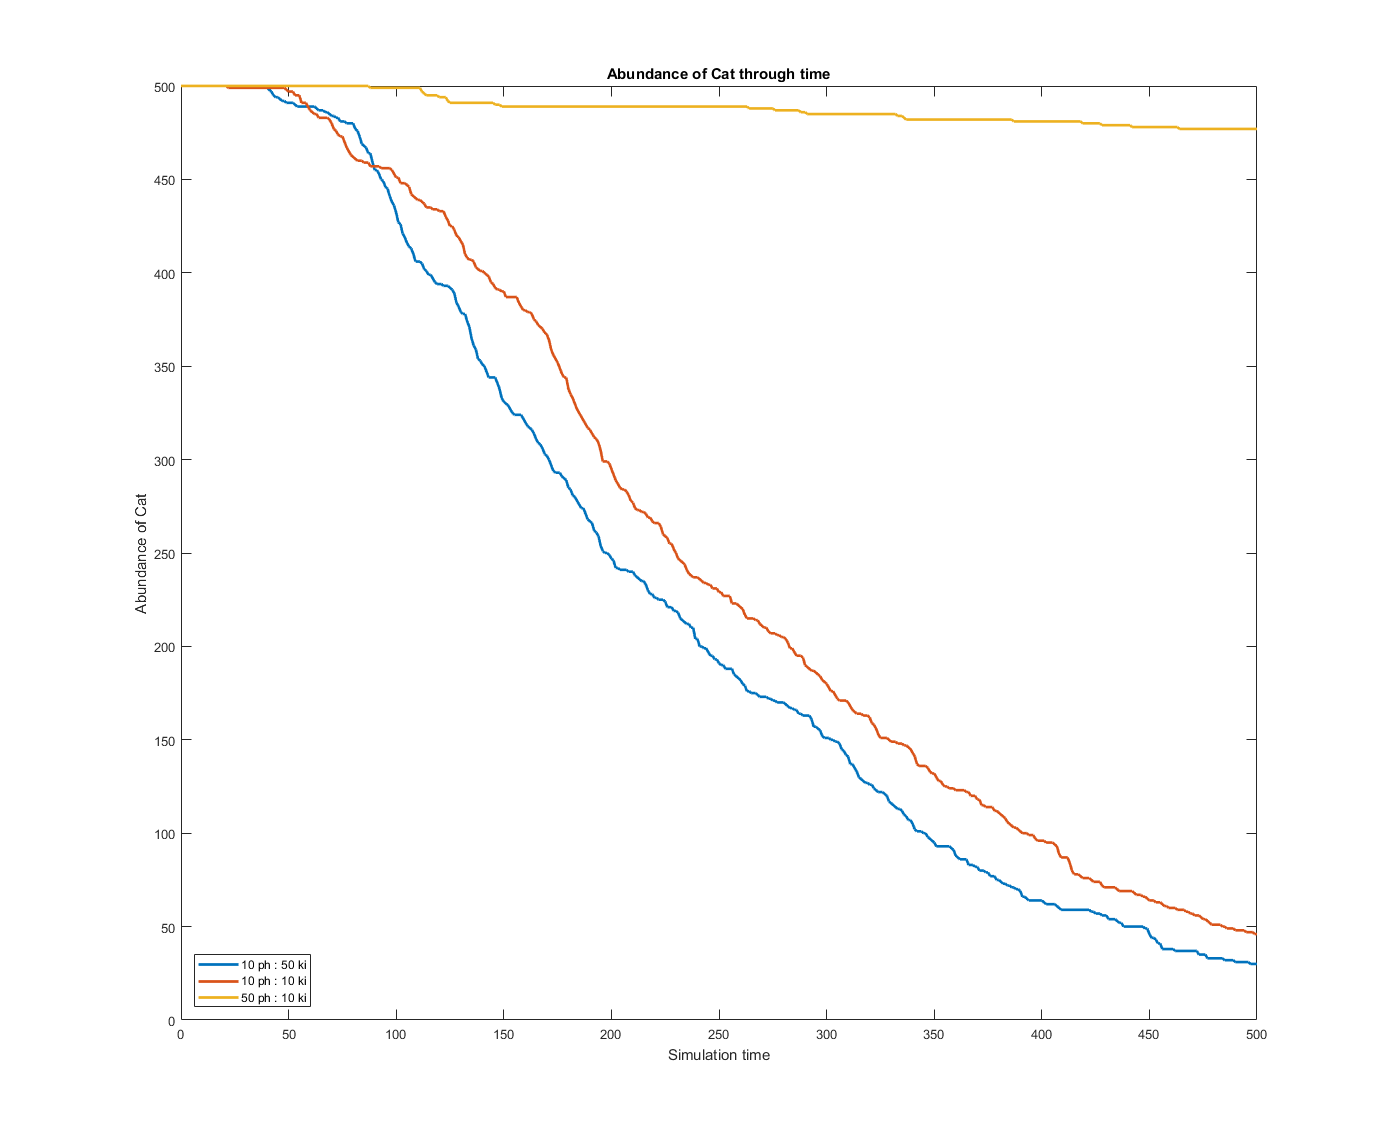
\includegraphics[width=\columnwidth]{wnt/F0_abundance_of_cat_through_time}
  \caption{Tracking the abundance of agent Cat through the
    simulation. At time $T=0$, the agents are introduced, all in
    monomeric form. The simulation was stopped after five hundred
    simulated seconds. In this legend and throughout the figures, ph
    stands for phosphatase, ki stands for kinase, and the agent
    numbers are presented. Thus ``$10$ ph : $50$ ki'' means the system
    with $10$ units of phosphatase and $50$ of kinase.}
  \label{F0}
\end{figure}


\subsubsection{Complex composition: all four on the same component?}

For the final query, we wonder if all four final phosphorylation
events occur on the same complex. Given the short wait time
(Figure~\ref{F2}), one might expect so, but the number of
dephosphorylation events is so large (Figure~\ref{F1}), it could be
well that a substrate is partially modified on one complex,
subsequently modified on another, finalized in yet another. Lacking a
metric by which we can compare complexes for distance, we instead
compare complex compositions as a proxy.

Seeing how overwhelmingly, for each specific modification on a single Cat, the
S45 phosphorylation events happened on complexes of the same Axn and
APC composition as the T41 phosphorylation events, as the S37
phosphorylation events, as the S33 phosphorylation events, we feel
confident in claiming all four steps occurred on the same
complex. This agrees well with the observation that the wait times are
fairly short (Figure~\ref{F2}). We did not see an appreciable
difference for the other parameter regimes.

\begin{figure}[p]
  \centering
  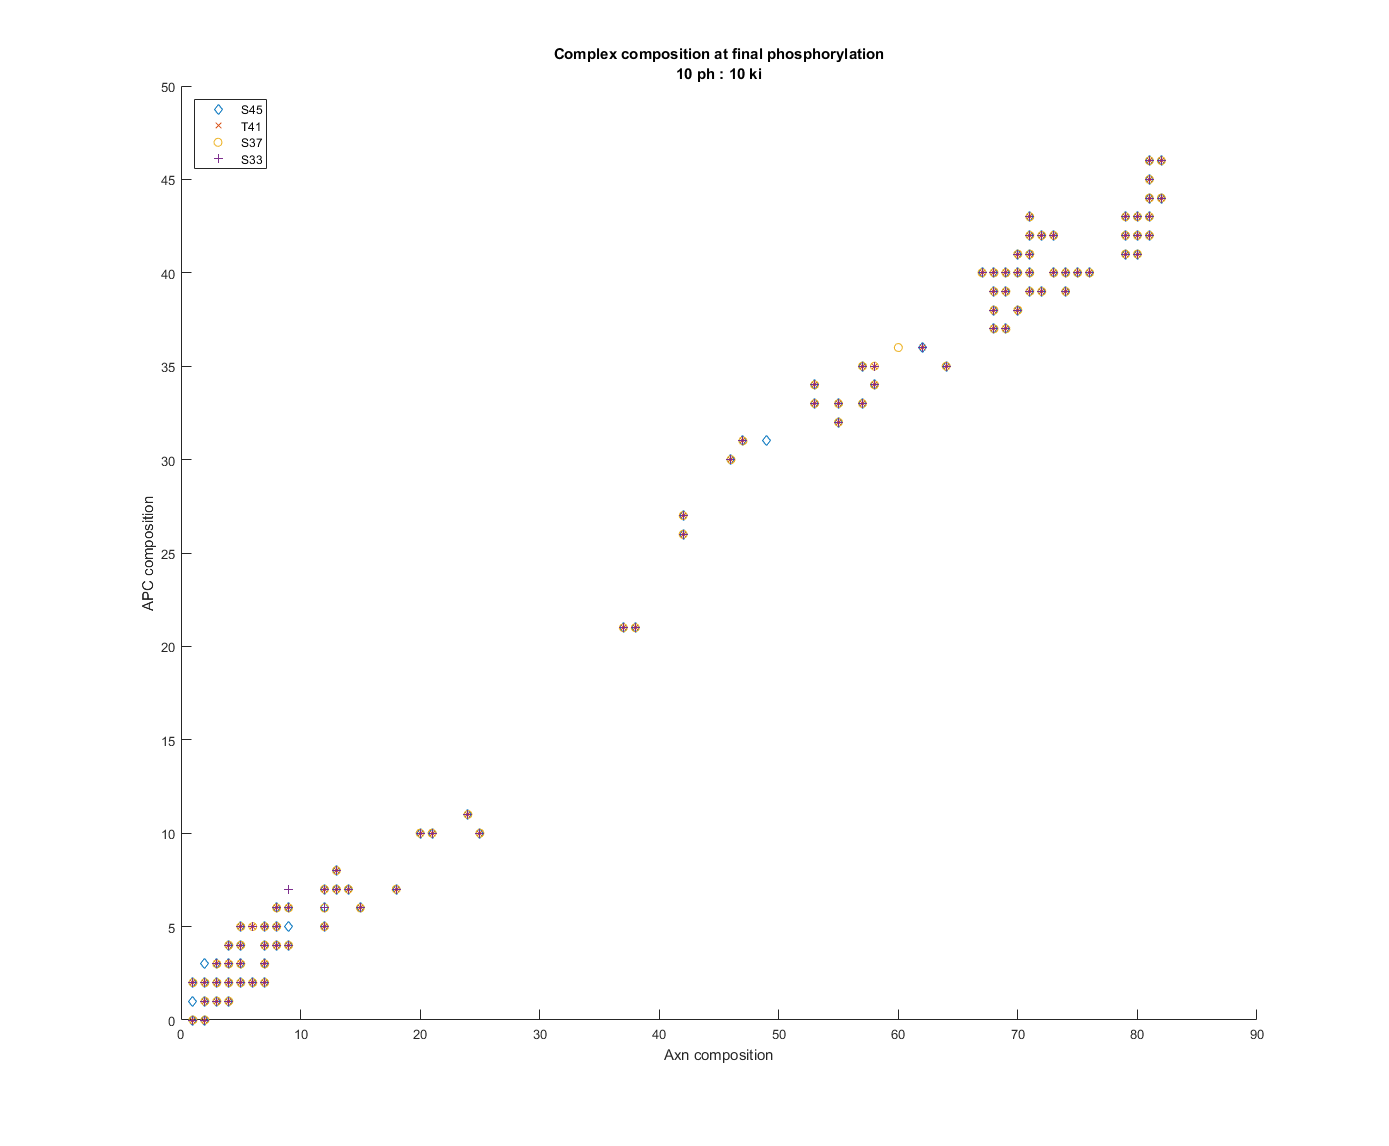
\includegraphics[width=\columnwidth]{wnt/F11_complex_composition_10_10}
  \caption{Complex composition at the time of the last phosphorylation
    for the 1:1 system. All four residues are shown. A diamond
    superposed with a cross superposed with a circle superposed with a
    plus sign indicates all four modifications for a specific copy of
    Cat occurred on a complex of the same composition in terms of Axn
    and APC. We interpret this as having occurred on the exact same
    complex.}
  \label{F11}
\end{figure}

\end{document}